% 使用 XeLaTeX 编译；所有章节及源码均为 UTF-8。
\documentclass[UTF8,a4paper,zihao=-4,oneside,fontset=fandol]{ctexrep}
\usepackage[margin=24mm,headheight=15pt]{geometry}
\usepackage{fontspec}
\setmonofont{Consolas}[Scale=0.88]
\usepackage{amsmath,amssymb,booktabs,longtable,tabularx,array}
\usepackage{graphicx,xcolor,tikz,float,caption,fvextra,fancyhdr,enumitem,needspace}
\usetikzlibrary{arrows.meta,positioning,shapes.geometric,calc}
\definecolor{ink}{HTML}{163B54}
\definecolor{pale}{HTML}{EDF3F6}
\definecolor{accent}{HTML}{2B7185}
\usepackage{xurl}
\usepackage[unicode,colorlinks,linkcolor=ink,urlcolor=accent,bookmarksnumbered]{hyperref}
\hypersetup{pdftitle={数据结构与算法专题实践：外存数据管理与归并排序实验报告},pdfauthor={刘酝潇}}
\ctexset{chapter={format=\Large\bfseries\color{ink},beforeskip=2pt,afterskip=18pt},section={format=\large\bfseries\color{ink}},subsection={format=\normalsize\bfseries}}
\setlength{\parskip}{3pt}
\linespread{1.23}
\setlist{nosep,leftmargin=2em,topsep=5pt}
\setlength{\emergencystretch}{3em}
\renewcommand{\arraystretch}{1.23}
\captionsetup{font=small,labelfont=bf,skip=7pt}
\pagestyle{fancy}\fancyhf{}
\fancyhead[L]{\small 外存数据管理与归并排序}
\fancyhead[R]{\small 课程实验报告}
\fancyfoot[C]{\thepage}
\renewcommand{\headrulewidth}{0.3pt}
\fancypagestyle{plain}{\fancyhf{}\fancyfoot[C]{\thepage}\renewcommand{\headrulewidth}{0pt}}
\newcolumntype{Y}{>{\raggedright\arraybackslash}X}
\newcommand{\code}[1]{\nolinkurl{#1}}
\newcommand{\src}[1]{\code{#1}}
\newcommand{\shot}[4]{\begin{figure}[H]\centering\includegraphics[width=\linewidth,trim=#4,clip]{figures/#1}\caption{#2}\label{#3}\end{figure}}
\tikzset{box/.style={draw=accent,rounded corners=2pt,fill=pale,align=center,font=\small,minimum height=10mm,text width=32mm},flow/.style={-{Stealth[length=2mm]},thick,draw=accent}}
\fvset{fontsize=\fontsize{8.6}{11}\selectfont,breaklines=true,breakanywhere=true,numbers=left,numbersep=7pt,xleftmargin=6mm,tabsize=4,frame=lines,framesep=3mm,rulecolor=\color{black!20},samepage=false}
\begin{document}
\begin{titlepage}\thispagestyle{empty}
\vspace*{12mm}
\begin{center}
{\zihao{1}\bfseries 东南大学}\par\vspace{12mm}
{\Large 数据结构与算法专题实践}\par\vspace{5mm}
{\color{accent}\rule{0.88\linewidth}{1.2pt}}\par\vspace{15mm}
{\zihao{2}\bfseries 外存数据管理与归并排序}\par\vspace{7mm}
{\zihao{2}\bfseries 实验报告}\par\vspace{10mm}
{\large Project 1\quad /\quad Project 2\quad /\quad Project 3}\par\vspace{24mm}
\begin{tabular}{rl}
学生姓名：& 刘酝潇\\[8pt]
学\hspace{2em}号：& 09024211\\[8pt]
课\hspace{2em}程：& 数据结构与算法专题实践\\[8pt]
实验主题：& 外存数据管理与归并排序\\[8pt]
实现语言：& C++11\\[8pt]
实验环境：& Windows 原生 MSVC / WSL2 GCC
\end{tabular}
\vfill {\large 2026 年 11 月}\par\vspace{8mm}
{\small 本报告采用自主排版，不代表学校官方模板。}
\end{center}\end{titlepage}
\pagenumbering{Roman}
\chapter*{摘要}\addcontentsline{toc}{chapter}{摘要}
本实验围绕有限工作内存条件下的整数外排序，完成从二进制文件组织到多路归并的连续工程实践。文件采用固定大小文件头、预留目录和顺序数据区，多个不等长有序段共存于同一文件。输入与输出缓冲将逐元素比较转换为分块读写，使算法不必持有完整数据。

Project 1以固定容量分块内排生成初始段，建立普通二叉归并计划并后序执行。Project 2用真正保存内部败者的败者树实现置换选择，通过冻结与解冻生成长段；输入、计算和输出采用双缓冲与三个线程的阶段同步，并以哈夫曼方法选择二路归并顺序。Project 3复用置换选择，在归并阶段维护共享的$2k$输入块、每路队列和空闲池，按最后已读关键字调度预取，完成真正的K路选择和多轮归并。

最终代码在Windows原生Debug和Release环境完成完整验收，测试包含220次与\code{std::sort}完整结果的精确比较、机制与非法输入检查以及6项CTest。真实实验中，$N=50003,M=256,B=64,k=4$时，初始段由196减为99，Project 3的数据块读写调用总数为7970，少于Project 1的13964；但在本次小块、可缓存的数据规模下，阶段线程创建和同步使并行方案耗时更高。报告区分理论搬移代价、应用层块调用和实际计时，说明这些结果的条件与边界。

本文按问题需求、系统结构、模块设计、测试分析、实验总结和完整源码六部分组织。运行截图来自Windows实际程序，性能图由保存的CSV生成；最后附全部17个正式C++文件及构建配置，源码快照与已验收提交对应。

\noindent\textbf{关键词：}外存排序；归并段；败者树；置换选择；动态缓冲；阶段同步
\tableofcontents\clearpage
\pagenumbering{arabic}
\chapter{问题描述与需求分析}
\section{问题背景与数据约束}
排序算法必须在内存中比较关键字，但实际文件可能远大于可用于排序的工作区。若把全部输入装入\code{vector}再调用内排序，空间需求随$N$增长，无法说明外存管理机制。本实验把原始数据保存在文件中，排序过程中每次只处理限定数量的整数，再把阶段结果写回文件。

外存算法的代价不仅是比较次数。逐个整数调用文件接口会产生大量细碎访问；将相邻值按块传输可以利用顺序访问，把一次I/O服务于多次比较。缓冲区因此承担两个不同粒度之间的衔接：文件按块读写，计算按元素取值或输出。操作系统仍可能缓存这些调用，故程序计数不等于硬盘实际寻道或物理读写次数。

归并段是文件中一个连续、内部非降序的整数序列。多个段分别有序，并不意味着按段号拼接后整体有序。算法先生成段，再反复合并，直到只剩一个逻辑最终段。实现保留旧段以便核验，因此“只剩一个”指当前参与归并的段号列表只剩一个，而非磁盘目录只剩一项。

\begin{table}[htbp]\centering\caption{全篇符号与单位}\label{tab:symbols}
\begin{tabularx}{\linewidth}{lY}\toprule
符号 & 含义\\\midrule
$N$ & 原始输入的整数总数，每个元素为\code{int32_t}。\\
$M$ & 分块内排或置换选择候选容量，以元素个数计。\\
$B$ & 一个数据块可容纳的整数数，常见平台字节容量为$4B$。\\
$k$ & 每组K路归并允许的最多路数，至少为2。\\
$R$ & 生成阶段产生的初始段数；$L_i$表示第$i$段长度。\\
$C$ & 二叉计划中所有内部节点长度之和，即理论合并输出元素量。\\
$S$ & 分阶段并行任务的同步阶段数量，不等同于归并轮数。\\\bottomrule
\end{tabularx}\end{table}

如表\ref{tab:symbols}所示，$M$不是整个进程的字节内存上限。缓冲区、败者树状态、目录、计划以及测试参考数组另占空间。正式排序入口\code{sortFile}接收文件路径，不接收完整数据数组；测试层为获得独立参考答案，可以持有完整输入及\code{std::sort}结果。二者的职责必须分清。

\section{课程要求及实现范围}
本报告以用户提供的《外存数据管理》课件、两份课堂语音转写和最终任务说明为课程依据。课件第75--81页给出Week 3--8推进顺序，分别覆盖文件与缓冲、归并计划、置换选择、动态缓冲、多路归并及测试评估。课堂说明要求最终报告附带有注释的源码，并能够解释重要函数和数据结构。

三项项目在同一仓库中逐步演进。矩阵文件示例用于理解Header、Directory和Data的组织思想；本实现将对象换为一维归并段。矩阵乘法、快排外排序、多块缓存替换和脏块机制不属于本次实现范围。这样的取舍使每一层都有明确输入输出，课堂演示可以直接追踪整数在文件、块和候选树之间的移动。

\section{Project 1：基于计划树的二路外排序}
Project 1首先解决可运行的完整外排序流程。输入是无文件头的连续本机字节序整数；输出是带目录的归并文件，以及说明最终段位置的\code{finalRun}。生成阶段每次读取不超过$M$个值，在内存中排序后按$B$写成一个有序段。由此得到至多$\lceil N/M\rceil$个初始段。

归并前先建立二叉计划。叶子引用已经存在的初始段，内部节点记录一次未来归并及两个孩子。计划构造与执行分开：先能打印整棵树、核对长度，再按后序递归执行。两路归并只保留两个输入块和一个输出块，不把两个完整段同时装入内存。奇数个节点时，最后一项带入下一层，避免无意义复制。

关键验收目标是：文件偏移正确、每个初始段及中间段有序、递归依赖正确、尾块不丢失、最终内容与参考排序逐项相同。仅显示“输出有序”不足以排除丢失或重复元素。

\section{Project 2：长段生成与置换选择}
普通分块生成的段长最多为$M$。若候选集合持续接纳仍能排在当前输出后面的新数，就有机会生成更长段，降低后续归并工作。Project 2维护固定$M$个候选，用败者树选出当前最小值，每输出一个再补入一个。若补入值小于刚输出值，则冻结，留给下一段；当前有效候选全部冻结时换段并解冻。

长段长度不等，因此归并顺序有实际影响。采用每次合并最短两段的哈夫曼计划，优化加权元素搬移量。并行发生于置换选择：输入线程预读备用块，计算线程操作活动块和树，输出线程写上一阶段的输出块。每阶段用\code{join}等待全部任务完成，再交接角色；后续二路归并仍为串行。

本项目必须体现真实败者数组、冠军路径更新、冻结状态、双输入/双输出以及段边界处理。不能以对全体数据排序替代置换选择，也不能仅启动空线程来声称完成并行。

\section{Project 3：K路归并与动态缓冲调度}
Project 3复用置换选择的初始段，归并阶段同时比较多路头值，使每轮段数按约$k$倍缩减。输入块不能永久固定为每路两个：各路消耗速度取决于关键字大小，某一路可能持续获胜，另一条路暂时不消耗。共享$2k$个物理块、各路队列和空闲池使空闲容量能够转给更需要的路。

预取依据是每路“最后一个已读关键字”，并在仍有未读数据的路中选择其最小者；缺少头值的空队列先补齐。未知头值意味着无法证明其他路当前值最小，因此必须在同步点等待补块。输出仍是一路，使用两块交替。多轮主控要正确处理不足$k$的末组、单段直接带过、空输入以及最终输出排空。

\begin{table}[htbp]\centering\caption{功能需求与验收依据}\label{tab:requirements}
\small\begin{tabularx}{\linewidth}{lYY}\toprule
需求 & 实现约束 & 可核验结果\\\midrule
文件组织 & 固定头、预留目录、流式追加 & 重开后偏移及数量正确，Scan/Put/Search有效\\
块缓冲 & 逐元素接口、尾块显式刷新 & 10个值、$B=3$时各4次数据块读写\\
二路计划 & 先建树、后序执行 & 15值示例4段、3次归并、$C=30$\\
置换选择 & $M$候选、冻结、败者路径重赛 & 15值示例段长7/7/1\\
最优计划 & 每次合并最短两段 & 7/7/1的代价由29减为23\\
阶段线程 & 三任务独占数据、join交接 & 输入/计算/输出有真实任务，最后一块排空\\
动态K路 & $2k$共享池、每路队列、跨路回收 & 测试中一路可占4块，回收块供另一条路使用\\
正确性 & 完整内容与参考排序一致 & 220次精确比较及机制断言通过\\
可演示性 & 原生构建、具名启动项、断点 & 一键十项验收与VS Code实测\\\bottomrule
\end{tabularx}\end{table}

\chapter{系统结构与算法思想}
\section{统一工程与分层关系}
工程只有一个\code{main.cpp}和一个可执行程序。命令行负责模式分派与验证，\code{sortFile}负责连接算法，文件层负责存储；败者树只处理候选，不依赖磁盘。图\ref{fig:architecture}概括这些调用关系。这种分层让三个项目共享底层机制，也便于独立检查某一层的错误。

\begin{figure}[htbp]\centering
\begin{tikzpicture}[node distance=10mm and 8mm]
\node[box,text width=125mm] (main) {main：参数解析、输入准备、结果验证};
\node[box,text width=125mm,below=of main] (sort) {sortFile：参数检查、目录预算、算法选择、统计计时};
\node[box,below=of sort] (p2) {Project 2\\置换选择 + 最优二叉计划};
\node[box,left=of p2] (p1) {Project 1\\分块内排 + 普通二叉计划};
\node[box,right=of p2] (p3) {Project 3\\置换选择 + 多轮K路归并};
\node[box,below=of p2,text width=125mm] (core) {InputBuffer / OutputBuffer\quad LoserTree\quad BufferPool};
\node[box,below=of core,text width=125mm] (file) {RawInput / RunFile：二进制文件、目录、块读写};
\draw[flow] (main)--(sort);\draw[flow] (sort)--(p2);
\draw[flow] (sort.south -| p1)--(p1);\draw[flow] (sort.south -| p3)--(p3);
\draw[flow] (p1)--(core.north -| p1);\draw[flow] (p2)--(core);\draw[flow] (p3)--(core.north -| p3);\draw[flow] (core)--(file);
\end{tikzpicture}\caption{系统结构与公共模块，箭头表示上层调用下层}\label{fig:architecture}\end{figure}

\code{RunFile}管理已经提交的目录和当前正在追加的段。算法返回目录下标，由调用者继续定位数据；这避免用“返回整个排序数组”的接口破坏外排序的空间约束。所有初始与中间结果顺序追加到同一个运行文件。目录中的旧段保持可读，当前归并列表决定哪些段参加下一轮。

\section{三个项目的数据流与复用}
\begin{table}[htbp]\centering\caption{三条完整数据处理路线}\label{tab:routes}
\begin{tabularx}{\linewidth}{lYYY}\toprule
环节 & Project 1 & Project 2 & Project 3\\\midrule
共同输入 & \multicolumn{3}{l}{原始本机字节序\code{int32_t}文件，经RawInput按块访问}\\
生成 & 固定$M$内排 & 败者树置换选择 & 复用置换选择\\
初始结果 & \multicolumn{3}{l}{RunFile中命名为R0、R1等的有序段}\\
计划/调度 & 相邻配对二叉树 & 最短两段优先二叉树 & 每轮按至多$k$段分组\\
执行 & 后序 + twoWayMerge & 复用后序 + twoWayMerge & kWayMerge + BufferPool\\
返回 & \multicolumn{3}{l}{新增最终段的目录下标finalRun，以及SortResult统计}\\\bottomrule
\end{tabularx}\end{table}

表\ref{tab:routes}体现了项目的递进关系。Project 2替换生成策略和计划策略，但沿用文件、缓冲及二路执行器；Project 3沿用长段生成与败者树，替换归并主控和输入块管理。K路阶段直接管理物理块队列，没有再为每一路永久配置两个\code{InputBuffer}对象。

以Project 2默认输入为例，\code{main}先写15个整数；\code{sortFile}计算目录容量为$2\lceil15/4\rceil+1=9$；数据起点为$32+9\times48=464$字节。置换选择生成长度7、7、1的段，最优计划先归并1与7，再归并8与7。最终\code{main}根据返回段号分块读取15个值，与独立参考排序逐个核对。

\section{主要源文件职责}
\begin{longtable}{p{46mm}p{102mm}}
\caption{模块、接口与调用关系}\label{tab:modules}\\\toprule 文件组 & 职责及连接方式\\\midrule\endfirsthead
\toprule 文件组 & 职责及连接方式\\\midrule\endhead
\code{main.cpp} & number严格解析数值，usage说明模式，main调用演示/测试或sortFile，再验证输出。\\
\code{run_file.h/.cpp} & FileHeader、RunInfo、IoStats、RunFile、RawInput；负责创建文件、目录查询、段追加及数据块访问。\\
\code{buffer.h/.cpp} & InputBuffer提供next；OutputBuffer提供writeValue和flush；连接逐元素算法与分块文件接口。\\
\code{merge_plan.h/.cpp} & runGeneration、MergeNode、MergePlan、两类建树、twoWayMerge及executeMergePlan。\\
\code{loser_tree.h/.cpp} & Candidate的valid/frozen/value状态；建树、取冠军、冠军路径重赛、解冻。\\
\code{replacement.h/.cpp} & 双输入与双输出、输出值的段号标签、三线程置换选择及跨段写入。\\
\code{kway_merge.h/.cpp} & InputBlock、BufferPool；预取选择、块生命周期、单组K路归并及多轮主控。\\
\code{projects.h/.cpp} & SortResult与sortFile，连接生成和归并策略，记录计时与计数。\\
\code{tests/test_sort.h/.cpp} & 机制断言、Week 3演示、220次精确对照、固定种子12行Benchmark。\\
\code{CMakeLists.txt} & C++11、线程库、警告选项、目标源文件以及6项CTest；不参与运行算法。\\\bottomrule
\end{longtable}

每组头文件定义类型及接口，\code{.cpp}给出实现。第\ref{chap:source}章列出全部17个正式C++文件，表\ref{tab:modules}按模块合并展示，不表示省略对应头文件或实现。Windows的一键脚本、CMake预设和VS Code配置属于验收支持层，不改变排序的模块边界。

\section{关键不变量与错误传播}
文件层保证已提交目录项描述连续且在文件范围内的数据；未完成段只存在于\code{pending_}，直到\code{endRun}更新目录。缓冲层保证$0\le pos\le count\le B$，只有有效范围被消费。候选树保证所有有效未冻结值优先于冻结值及无效叶，冠军始终代表当前允许输出的最小值。

并行层强调阶段内所有权：输入线程写预留块，计算线程操作已公开块，输出线程只读上一阶段输出。三个任务的异常分别存入\code{errors[3]}，主线程全部\code{join}后才读取并重抛。若后续线程创建失败，也先回收已启动线程，再向顶层报告，避免可连接线程在析构时终止进程。

\section{Git演进与可复现交付}
仓库\url{https://github.com/David-JayTao/Experiment-External-Memory-Sorting}保存一个持续演进工程。\code{week3-complete}至\code{week8-complete}对应功能检查点：文件缓冲、二路计划、长段、动态池、K路主控、最终测试。标签保留当时源码和支持的命令，不将当前所有功能倒写到早期版本，也不改动真实提交时间。

Windows配置与中文注释分别形成独立中文提交。源码附录从最后验收版本自动生成，版本号写在第\ref{chap:source}章。个人姓名、学号及正式报告保存在本地被忽略的\code{report/}目录；公开仓库只保留源码及通用验收资料。复现报告只需该目录中的LaTeX、截图、CSV、矢量图和代码快照，不需要编译产物或安装包。

\chapter{功能模块设计}
\section{二进制文件组织}
\subsection{物理布局与定位公式}
\code{FileHeader}用32字节保存标识、目录容量、已提交段数以及目录和数据起点。\code{RunInfo}用48字节保存32字节名称、64位字节偏移与64位元素数量。编译期\code{static_assert}检查结构大小；文件直接保存这些结构的本机表示，不声称能跨字节序交换。

\begin{figure}[htbp]\centering
\begin{tikzpicture}
\node[box,text width=23mm,minimum height=17mm] (h) at (0,0) {Header\\32字节};
\node[box,text width=51mm,minimum height=17mm,right=2mm of h] (d) {Directory\\$48\times maxRuns$字节};
\node[box,text width=47mm,minimum height=17mm,right=2mm of d] (data) {Data\\R0、R1、M/K中间段};
\node[below=2mm of h,font=\small] {起点0};
\node[below=2mm of d,font=\small] {起点32};
\node[below=2mm of data,font=\small] {$32+48\times maxRuns$};
\end{tikzpicture}\caption{归并文件物理布局；目录预留区大小在创建时固定}\label{fig:file-layout}\end{figure}

图\ref{fig:file-layout}中目录容量与已用数量分开。预留目录保证后续追加一项不会挤占原数据区。第$i$段内零起始下标$p$的整数位于
\begin{equation}
\operatorname{address}(i,p)=\operatorname{RunInfo}[i].offset+p\cdot\operatorname{sizeof}(int32\_t),\quad 0\le p<count_i.
\end{equation}
段号、段内元素下标和文件字节偏移是三个不同概念。\code{readBlock}先检查段号，再计算实际数量$\min(B,count_i-p)$，定位并读取；$p=count_i$返回0，$p>count_i$拒绝。每次读写都重新\code{seekg/seekp}，不依赖上一次操作留下的流位置。

\subsection{Scan、Put、Search与流式提交}
\code{scan()}返回已加载的目录常量引用，遍历目录不会自动加载段数据；\code{search(name)}逐项比较名称，找到返回目录下标，否则返回$-1$。\code{put(name,values)}是小数据的便利包装，适合Week 3与机制测试。正式长段采用表\ref{tab:append}中的流式接口。

\begin{table}[htbp]\centering\caption{一次归并段追加的状态变化}\label{tab:append}
\begin{tabularx}{\linewidth}{lYY}\toprule
调用 & 前置条件与行为 & 状态结果\\\midrule
beginRun & 可写、无待写段、目录未满、名称合法且不重复 & pending记录名称与endOffset，writing为true\\
writeBlock & 已开启段，追加count个整数；空块跳过 & pending.count加count，endOffset加$4count$\\
endRun & 调用方先刷新尾块，再写目录与头部并flush & 更新runCount、加入runs，返回新目录下标\\\bottomrule
\end{tabularx}\end{table}

数据先写、目录后提交，使读取者只通过已完成目录访问完整段。\code{endRun}显式刷新并检查流状态，随后另开只读文件可以看到结果；但它不是掉电原子事务。打开文件时检查标识、目录边界、段连续性和数据范围，能发现常见截断或损坏，不等于完整的恶意输入安全解析器。

Week 3创建容量8的目录，数据从416字节开始。A为$[-5,2,8]$，占12字节；B为$[0,1]$，起点428；C为$[3,4,5,6,7]$，起点436。重新打开后逐块输出仍应相同，Search C得到2，missing得到$-1$。这一例子同时检查物理偏移与目录语义。

\section{输入与输出缓冲区}
\code{InputBuffer}绑定一个段和一个容量为$B$的数组，维护\code{nextOffset_}、\code{pos_}、\code{count_}。\code{next}在$pos=count$时补下一块，推进段内下一读取位置并把$pos$清零；读到0说明段耗尽，否则把一个整数通过引用参数交给调用者。长度7、$B=3$时，底层返回数量依次为3、3、1、0，只有前三次增加读计数。

\code{OutputBuffer}维护有效数量，\code{writeValue}填一个值，达到$B$立即\code{flush}；最后不足$B$的尾块由调用者显式刷新，再提交段。析构不隐式写盘，避免把可能抛出错误的I/O藏在资源销毁过程中。连续调用空刷新不会产生额外非空块计数。

\begin{figure}[htbp]\centering
\begin{tikzpicture}[node distance=7mm]
\node[box,text width=26mm] (a) {段文件\\按块读};
\node[box,text width=28mm,right=of a] (b) {InputBuffer\\逐个next};
\node[box,text width=23mm,right=of b] (c) {比较与选择};
\node[box,text width=30mm,right=of c] (d) {OutputBuffer\\满块/尾块写};
\draw[flow](a)--(b);\draw[flow](b)--(c);\draw[flow](c)--(d);
\end{tikzpicture}\caption{缓冲区连接块传输与逐元素计算，输出再追加到段文件}\label{fig:buffer-flow}\end{figure}

图\ref{fig:buffer-flow}中的封装让二路归并只考虑当前值和有效性，而无需在比较循环中重复写补块逻辑。\code{IoStats*}可为空，验证层由此不把额外扫描算入排序指标。缓冲对象借用文件引用，文件应在对象使用期间始终存活。

\section{固定容量初始归并段生成}
\code{runGeneration(rawPath,file,M,B,stats)}用一个长度$M$的数组。每轮按不超过$B$的块读取，直到凑满$M$或文件结束；只对有效范围调用\code{std::sort}，随后用输出缓冲逐个写出，刷新并提交为\code{R0}、\code{R1}等。返回的是段号序列，不是数据副本。

\begin{enumerate}
\item 令当前有效数为0，按$\min(B,M-count)$读取到工作数组剩余位置。
\item 若实际读入总数为0则结束；否则在$[0,count)$内排序。
\item 开启新段，按$B$写完已排序值，尾块刷新后提交目录。
\item 重复直至原始输入耗尽；空输入不生成空初始段。
\end{enumerate}

默认输入$[9,1,8,2,7,3,6,4,5,0,-1,3,12,2,10]$取$M=4$得到表\ref{tab:initial}。每个长度4的段在$B=3$时分两次写，不能把段数或段长度误认为I/O块数。

\begin{table}[htbp]\centering\caption{Project 1默认输入的初始段}\label{tab:initial}
\begin{tabular}{clrr}\toprule 段 & 排序后内容 & 元素数 & 字节起点\\\midrule
R0 & 1, 2, 8, 9 & 4 & 464\\
R1 & 3, 4, 6, 7 & 4 & 480\\
R2 & $-1$, 0, 3, 5 & 4 & 496\\
R3 & 2, 10, 12 & 3 & 512\\\bottomrule
\end{tabular}\end{table}

比较成本为$O(N\log M)$，工作数组及输出块为$O(M+B)$，另有$O(R)$段号及目录。若$M$不整除$B$，每个工作区末次读取可能不足块；真实调用数要逐段取整，不能直接等同于$\lceil N/B\rceil$。

\section{二路归并与二叉计划执行}
\subsection{节点表示与普通计划}
\code{MergeNode}包含左右孩子下标、实际段号与长度。叶子孩子为$-1$，段号已知；内部节点的段号初始为$-1$，执行后记录结果。\code{MergePlan}保存节点数组、根和代价。建树先放叶子，再逐层相邻配对，所以孩子下标小于父节点，根在末尾。

图\ref{fig:binary-tree}是表\ref{tab:initial}对应的真实计划，方框中表示节点下标与长度。节点4先合并0与1，节点5合并2与3，最后根6合并4与5。建树仅访问目录，真正的数据I/O发生于后序执行。

\begin{figure}[htbp]\centering
\begin{tikzpicture}[level distance=13mm,sibling distance=65mm,every node/.style={draw=accent,fill=pale,rounded corners,align=center,font=\small},edge from parent/.style={draw=accent,thick}]
\node {6：长度15}
child {node {4：长度8} child[sibling distance=29mm]{node {0：R0\\长度4}} child[sibling distance=29mm]{node {1：R1\\长度4}}}
child {node {5：长度7} child[sibling distance=29mm]{node {2：R2\\长度4}} child[sibling distance=29mm]{node {3：R3\\长度3}}};
\end{tikzpicture}\caption{普通归并计划的具体节点与依赖，总代价$8+7+15=30$}\label{fig:binary-tree}\end{figure}

\subsection{后序执行与两路选择}
\code{executeMergePlan}遇到根$-1$返回$-1$；遇到已有段号的节点直接返回；否则先递归完成左、右子树，将返回的两个段号交给\code{twoWayMerge}，把新段号写回当前节点。缓存结果保证同一计划节点不会被重复执行。递归栈只保存少量状态，不保存各层完整数据。

\code{twoWayMerge}建立左右输入缓冲和一个输出缓冲，用\code{hasLeft/hasRight}区分合法值与结束。每次输出较小头值，只推进对应输入；相等优先左路，一方耗尽后排空另一方。结果仍以新段追加到同一文件。这里使用同一个\code{fstream}是安全的，因为两路读取和写入都在同一线程顺序执行。

若左右长度为$a,b$，CPU比较/移动为$O(a+b)$，整数缓冲为$3B$。一次归并数据块调用数为
\begin{equation}
Q_{\rm merge}=\left\lceil\frac{a}{B}\right\rceil+\left\lceil\frac{b}{B}\right\rceil+\left\lceil\frac{a+b}{B}\right\rceil.
\end{equation}
这里不包含文件头与目录读写。正确性可由不变量说明：输出前缀已排序，且其中每个元素不大于两路剩余值；取较小头值保持这一性质，最终数量为$a+b$。

\section{败者树的结构与更新规则}
败者树叶子是\code{Candidate(value,valid,frozen)}。内部数组\code{losers_}保存每场比赛的败者叶下标，总冠军另存\code{champion_}。候选数补齐至2的幂，多出的叶子标为无效，不占真实候选名额。\code{valid=false}代表EOF或补齐叶，避免用\code{INT_MAX}哨兵排除真实最大整数。

比较顺序为有效优先、未冻结优先、数值小优先、叶下标小优先。\code{build}从子树取得两个冠军，将败者留在当前内部节点，赢家向父亲返回。\code{winner}若发现总冠军无效便返回$-1$；\code{top}只在仍有冠军时作为有效输出使用。

\begin{figure}[htbp]\centering
\begin{tikzpicture}[level distance=13mm,sibling distance=62mm,every node/.style={draw=accent,fill=pale,align=center,font=\small,rounded corners},edge from parent/.style={draw=accent}]
\node {内部1存叶3（值2）\\总冠军：叶1（值1）}
child {node {内部2存叶0（值9）} child[sibling distance=27mm]{node {叶0：9}} child[sibling distance=27mm]{node {叶1：1}}}
child {node {内部3存叶2（值8）} child[sibling distance=27mm]{node {叶2：8}} child[sibling distance=27mm]{node {叶3：2}}};
\end{tikzpicture}\caption{候选$[9,1,8,2]$的败者树；内部持久存储的是败者下标}\label{fig:loser}\end{figure}

图\ref{fig:loser}中输出1后用7替换叶1。7先与记录的9比较获胜，再与记录的2比较失败，根留下叶1，总冠军改为叶3。只需沿被替换冠军的叶到根路径重赛，因为其他子树的比赛没有变化。该接口不能直接更新任意非冠军叶；本项目两处调用都符合“输出冠军后补入”的条件。

建树与批量解冻重建均为$O(M)$，单次冠军替换为$O(\log M)$。在K路归并中把$M$换为实际路数。平局按叶下标处理使演示确定，但本项目只排序整数，没有携带记录身份来承诺任意记录的全局稳定性。

\section{置换选择与冻结机制}
\subsection{从固定候选到长归并段}
\code{replacementSelection}先按块装入至多$M$个候选，构造败者树，再预载活动输入。每输出一个冠军，从活动输入补一个新值。如果新值不小于刚输出值，则仍能接在当前非降序段后；若更小，则保留在候选中并冻结。所有有效候选均被冻结时，总冠军也会被冻结，程序增加段号并\code{thaw}。

\begin{table}[htbp]\centering\caption{默认15值输入的第一段置换过程，$M=4$}\label{tab:replacement}
\begin{tabular}{rrll}\toprule 输出 & 补入 & 新候选状态 & 解释\\\midrule
1 & 7 & 活动 & $7\ge1$\\
2 & 3 & 活动 & $3\ge2$\\
3 & 6 & 活动 & $6\ge3$\\
6 & 4 & 冻结 & $4<6$，不能接入当前段\\
7 & 5 & 冻结 & $5<7$\\
8 & 0 & 冻结 & $0<8$\\
9 & $-1$ & 冻结 & 全部有效候选冻结，结束R0\\\bottomrule
\end{tabular}\end{table}

表\ref{tab:replacement}得到R0=$[1,2,3,6,7,8,9]$。解冻后生成R1=$[-1,0,3,4,5,10,12]$，再生成R2=$[2]$。三个段长为7、7、1，偏移为464、492、520。输入中重复值通过严格小于判断保留在当前段，不会因相等而不必要地冻结。

对于升序输入，新数持续满足条件，有可能只生成一个长段；对于逆序输入，新数频繁冻结，不能保证长于$M$。随机输入常出现平均接近$2M$的段长，但这依赖分布和模型，本实现不把它作为任意输入的长度保证。

\subsection{段边界、暂时缺块与真正结束}
输出内存块可能跨段，\code{GeneratedBlock}因此同时保存\code{values}和逐元素\code{runNumbers}。默认$B=3$时第三块为$[9,-1,0]$，段号为$[0,1,1]$。\code{writeGeneratedBlock}把它拆成同段连续区间，先写9并提交R0，再开启R1写$[-1,0]$。一个内存块由此可能对应多次数据写调用。

计算线程区分两种状态：活动输入块暂时耗尽但后面仍有数据，应结束本阶段等待；原始输入真正全部读完，才用无效候选逐个替换并排空树。阶段开始的\code{noMoreAfterActive}是由主线程确定的快照，避免计算线程读取输入线程正在修改的备用块计数。

即使树已空，上一阶段输出仍可能未写盘。循环条件必须同时检查树和待写输出，最后再关闭仍打开的段。这个排空规则与显式尾块刷新共同保证数量不丢失。

\section{三线程分阶段并行与双缓冲}
\subsection{阶段内的数据所有权}
置换选择有两输入块和两输出块。\code{activeInput}供计算消费，另一个输入块供预取；\code{activeOutput}供计算填充，另一个输出块供写回。两个索引只在主线程完成三个\code{join}之后更新。图\ref{fig:stages}展示稳定阶段的任务分工。

\begin{figure}[htbp]\centering
\begin{tikzpicture}[x=1cm,y=1cm]
\foreach \y/\t in {0/输入线程,-0.9/计算线程,-1.8/输出线程}{\node[anchor=east,font=\small] at (0,\y){\t};}
\foreach \x/\label in {0.2/阶段$t$,4.1/阶段$t+1$}{
\node[font=\small\bfseries] at (\x+1.65,0.65){\label};
\draw[fill=pale,draw=accent] (\x,-0.3) rectangle ++(3.3,0.6);
\draw[fill=pale,draw=accent] (\x,-1.2) rectangle ++(3.3,0.6);
\draw[fill=pale,draw=accent] (\x,-2.1) rectangle ++(3.3,0.6);}
\node[font=\small] at (1.85,0){读备用输入};\node[font=\small] at (1.85,-0.9){读活动输入，填$O_a$};\node[font=\small] at (1.85,-1.8){写上一阶段$O_b$};
\node[font=\small] at (5.75,0){按需补空输入};\node[font=\small] at (5.75,-0.9){继续选冠军，填$O_b$};\node[font=\small] at (5.75,-1.8){写已完成$O_a$};
\draw[dashed,thick,accent] (3.8,0.35)--(3.8,-2.5);
\node[below,align=center,font=\small] at (3.8,-2.5){三个join完成\\主线程交接角色};
\end{tikzpicture}\caption{三线程的阶段同步；输入仅在耗尽时切换，输出每阶段交替}\label{fig:stages}\end{figure}

\begin{table}[htbp]\centering\caption{阶段内可写状态与同步后的处理}\label{tab:ownership}
\small\begin{tabularx}{\linewidth}{lYY}\toprule 执行者 & 置换选择 & K路归并\\\midrule
输入线程 & 原始读流、备用输入块、readBlocks & 独立只读source、预留物理块、readBlocks\\
计算线程 & 树、活动输入位置、活动输出、currentRun & 树、消费队列、released、活动输出、emitted\\
输出线程 & 上阶段输出、段文件、writtenRun、writeBlocks & 上阶段输出、段文件、writeBlocks\\
主线程 & join后累加loaded、按需换输入、换输出 & join后归还块、发布预取块、换输出\\\bottomrule
\end{tabularx}\end{table}

表\ref{tab:ownership}说明无需在本实现中引入互斥锁的原因：阶段内可写对象不重叠，主线程不提前观察正在写的数据。输入和输出分别修改\code{IoStats}中不同标量成员；阶段数仅在join后更新。日志也限定由计算线程或同步后的主线程输出。

\subsection{交接顺序与异常收尾}
活动输入不一定在每个阶段都恰好用完，例如输出已满时还留有未消费输入。程序只有在$pos=count$时清空该块并切换，避免无条件换块跳过数据。输出线程处理完旧块后，主线程清空它，作为下一阶段的计算输出。

每阶段新建三个\code{std::thread}，随后逐个join。它们可以并行执行，但某个阶段可能没有预取任务或没有上一块可写，启动和排空阶段尤其如此。这个实现服务于课程的阶段同步机制，不是持续运行的线程池。阶段总耗时受最慢任务、线程创建以及调度影响，不能简单把单线程时间除以三。

线程内部异常必须捕获到各自的\code{exception_ptr}槽；主线程join之后再重抛。对线程创建失败的路径也保留已启动线程的join收尾。测试未故意耗尽系统线程资源，因此报告只声明该分支经代码审查，不将正常测试冒称为已覆盖此类系统故障。

\section{哈夫曼最优归并计划}
\code{buildOptimalPlan}将每个段转换为叶子，将$(length,nodeIndex)$放入最小优先队列。每次弹出两个最短节点，建立长度为两者之和的父节点，并重新入队，直到剩下根。等长时用节点下标确定先后，计划可重复。

设初始段$i$经过$d_i$次归并，则每个元素被复制$d_i$次，总代价满足
\begin{equation}
C=\sum_{v\text{为内部节点}}L_v=\sum_{i=1}^{R}L_i d_i.
\end{equation}
哈夫曼方法优化这一加权路径长度。它并不直接优化尾块取整、目录访问、缓存行为或CPU时间，因此最优计划不等于实际计时总是最快。

\begin{figure}[htbp]\centering
\begin{tikzpicture}[every node/.style={font=\small,align=center},edge from parent/.style={draw=accent},level distance=12mm]
\node at (-3.1,0) {普通：15}
 child[sibling distance=26mm]{node {14} child[sibling distance=17mm]{node {R0：7}} child[sibling distance=17mm]{node {R1：7}}}
 child[sibling distance=26mm]{node {R2：1}};
\node at (3.1,0) {最优：15}
 child[sibling distance=26mm]{node {R1：7}}
 child[sibling distance=26mm]{node {8} child[sibling distance=17mm]{node {R2：1}} child[sibling distance=17mm]{node {R0：7}}};
\node at (-3.1,-3.1){$C=14+15=29$};\node at (3.1,-3.1){$C=8+15=23$};
\end{tikzpicture}\caption{实际段长7、7、1的两种计划，执行器均复用二路后序归并}\label{fig:huffman}\end{figure}

图\ref{fig:huffman}中最优计划先生成长度8的M3，再生成长度15的M4。独立机制测试另用段长1、2、3、100验证普通代价212、最优代价115，防止只凭一次演示判断建树正确。建树的CPU成本为$O(R\log R)$，节点和优先队列为$O(R)$。

\section{真正K路选择与多轮归并}
\subsection{单组归并的阶段主循环}
\code{kWayMerge(file,runs,k,B,stats,trace)}接收至多$k$个段号，复制本组元数据并求总长度，另开只读\code{RunFile source}，初始化共享池，在原文件开启新K段。读线程访问已完成段，写线程追加后续区域，两个线程不共享同一个\code{fstream}对象。

\begin{figure}[htbp]\centering
\begin{tikzpicture}[node distance=6mm]
\node[box,text width=117mm] (a){初始化各路首块，开启输出段，emitted=0};
\node[box,text width=117mm,below=of a] (b){选预取路并保留空闲块；收集已公开头值，重建败者树};
\node[box,text width=117mm,below=of b] (c){输入读预留块 / 计算选最小并填活动输出 / 输出写上一块};
\node[box,text width=117mm,below=of c] (d){三个join；回收耗尽块；公开预取块；交换输出};
\node[box,text width=117mm,below=of d] (e){未输出完或还有待写块：继续；否则endRun返回段号};
\draw[flow](a)--(b);\draw[flow](b)--(c);\draw[flow](c)--(d);\draw[flow](d)--(e);
\draw[flow](e.west)--++(-0.5,0)|-(b.west);
\end{tikzpicture}\caption{K路归并阶段流程，循环末尾必须包含写出最后一块}\label{fig:kflow}\end{figure}

图\ref{fig:kflow}中的计算任务不是多次二路归并。它把实际各路头值组成一棵败者树，每输出一个冠军，消费该路一个值，再用该路新头替换冠军。若某条尚未结束的路暂时没有头值，\code{missingHead}使本阶段等待补块；若消费过程中出现这种状态，也立即结束本阶段计算。忽略未知头值会破坏全局最小值判断。

实现每阶段重新构造头值树，以纳入同步后公开的新块；阶段内部才使用冠军路径重赛。因此复杂度必须包括每阶段$O(k)$建树和扫描，不能只写理想的$O(N\log k)$。每阶段最多产生$B$个值，缺头时可能少于$B$，尾输出也需完整写出。

\subsection{多轮主控与不足K路的末组}
\code{mergeKRuns}把当前段号每$k$个分组；组内至少两个时调用一次K路归并，单个段直接带入下一轮。一次归并产生一个新段，但磁盘上的旧段保持不变。段号列表替换后继续，直到只剩一个；空输入返回$-1$。

例如实际99段、$k=4$时，段数为$99\to25\to7\to2\to1$，共4轮。归并组数为$25+6+2+1=34$：第二轮25段的最后单段直接带过，并不新增一次合并。\code{rounds}是多轮主控次数，\code{merges}是产生新段的归并组数，\code{stages}是线程同步阶段，三者不可互换。

\section{动态输入缓冲池与预取策略}
\subsection{物理块与逻辑队列分离}
\code{BufferPool.blocks_}一次分配$2k$个物理块，每块有整数数组、有效数量和消费位置。\code{queues_[lane]}只保存块号，\code{free_}保存可再分配块，\code{released_}暂存本阶段刚耗尽的块。\code{next_}记每路已读数量，\code{lengths_}是总长度，\code{lastKeys_}是所有已读数据的末值。

\begin{figure}[htbp]\centering
\begin{tikzpicture}[node distance=7mm]
\node[box,text width=106mm] (all){物理池：块0、1、2、3、4、5（$k=3$，每块容量$B$）};
\node[box,text width=31mm,below=of all] (q1){路1队列：[1]};
\node[box,text width=31mm,left=5mm of q1] (q0){路0队列：[0,3]};
\node[box,text width=31mm,right=5mm of q1] (q2){路2队列：[2]};
\node[box,text width=106mm,below=of q1] (free){空闲：[4,5]\quad 已消费块经join后归还，下一阶段可跨路使用};
\draw[flow](all)--(q1);\draw[flow](all.south -| q0)--(q0);\draw[flow](all.south -| q2)--(q2);
\draw[flow](q0.south)--(free.north -| q0);\draw[flow](q2.south)--(free.north -| q2);
\end{tikzpicture}\caption{默认示例第一个K路计算阶段同步后的队列状态}\label{fig:pool}\end{figure}

图\ref{fig:pool}中物理块和路没有永久绑定。初始化为每个非空段读一块，其余块保留为空闲；下一次预取用\code{reserve}取出一个块。读线程只填该块，join后\code{finishPrefetch}才把块号入队并更新\code{next_}和\code{lastKeys_}。消费块由计算线程出队，但仅登记到\code{released_}，主线程同步后统一归还，避免块仍被读取时就被重写。

\subsection{预取选择与真实跨路回收}
正常预取规则可写为
\begin{equation}
\operatorname{target}=\arg\min_{i:\ next_i<length_i}\operatorname{lastKeys}_i,
\end{equation}
并附加“仍有磁盘数据的空队列优先”规则。\code{lastKeys}不是队首最小值，也不是尚未读取的整段最大值；它由最近完成读取的块末值更新。已经全部读入的路不再预取，即使其队列尚有很多未消费数据。

默认三路首块分别为$[1,2,3]$、$[-1,0,3]$、$[2]$。路2已全部读入；路0、1末值相同，先选路0读$[6,7,8]$，之后选末值仍为3的路1。路2的物理块2被消费后回收，后续日志出现\code{prefetch lane=1 block=2}，用来读取路1的最后值12。这是实际跨路复用，不是仅在结构命名上叫“动态池”。

独立测试还让路0占有4个物理块、其他两路各占1块，共6块，证明并非永久每路两个。当没有可用块时\code{reserve}返回$-1$，本阶段不执行预取；计算继续释放块后再尝试。调度强调正确交接，不对所有系统时序承诺零等待。

\section{复杂度、内存与I/O成本}
\begin{longtable}{p{35mm}p{61mm}p{51mm}}
\caption{核心算法的CPU与额外内存成本}\label{tab:complexity}\\\toprule
模块 & CPU成本与条件 & 额外内存\\\midrule\endfirsthead
\toprule 模块 & CPU成本与条件 & 额外内存\\\midrule\endhead
固定分块生成 & $O(N\log M)$，段数$\lceil N/M\rceil$ & $O(M+B)$整数工作区，另有$O(R)$元数据\\
普通二叉计划 & $O(R)$建树；后序遍历$O(R)$，数据合并总计$O(C)$ & $O(R)$节点，递归深度通常$O(\log R)$\\
哈夫曼计划 & $O(R\log R)$建树；执行总数据处理$O(C)$ & $O(R)$节点和队列，最坏树深$O(R)$\\
单次二路归并 & 长度$a,b$时$O(a+b)$ & $3B$个整数及常量状态\\
败者树 & 建树/解冻$O(M)$，一次更新$O(\log M)$ & $O(M)$候选和败者下标\\
置换选择 & $O(N\log M+RM)$，另有$S$次阶段调度 & $O(M+B)$，含双输入、双输出及段号标签\\
K路单组归并 & 总长度$T$时$O(T\log k+S_g k)$，$S_g$为本组阶段数 & $O(kB+k)$，含$2k$输入和2输出块\\
预取及块管理 & 每阶段选择$O(k)$；每个块入队、出队、回收均摊$O(1)$ & 队列和状态$O(k)$，块数据计入上项\\\bottomrule
\end{longtable}

表\ref{tab:complexity}区分了核心算法与实现附加项。\code{beginRun}为检查重名进行线性目录查询，累计创建$D$段可能引入$O(D^2)$名称比较；K路每次另开只读RunFile还会读取当前目录。\code{sortFile}在Project 3也构造一次普通计划用于cost指标。这些元数据工作没有出现在理想归并的比较模型里，但属于实际运行时间。全部目录和历史计划仍需$O(R)$内存，不能宣称整个进程空间恒定。

忽略部分块、元数据及系统缓存，若每轮将全部$N$个值读写一次，初始段数为$R$，K路归并层数约为$L=\lceil\log_k R\rceil$，理想数据传输约为
\begin{equation}
Q_{\rm ideal}\approx 2\frac{N}{B}(1+L).
\end{equation}
首个1代表生成段的一读一写。真实实现有单段带过、各段尾块、置换输出跨段分拆、K路缺头提前结束阶段，因此应以\code{readBlocks/writeBlocks}为应用层调用的实测依据。最优树的$C$衡量元素量，也不能未经换算直接称为块I/O。

内存比较亦有条件：二路归并使用$3B$整数块，K路使用$(2k+2)B$，即使各项目设置同样$M,B$也不是同一总字节预算。哈夫曼减少搬移、置换选择减少段数、K路减少轮数，各自优化不同环节；线程创建与join、缓存、文件系统会共同决定最终耗时。

\chapter{测试结果与分析}
\section{测试环境与版本}
实验开发与Windows验收于2026年11月9--10日进行，报告整理延续至11月11日。表\ref{tab:env}分别列出Windows原生环境与此前WSL环境。两者的编译器、文件系统和计时不同，不能将其数据混为同一次实验。

\begin{table}[H]\centering\caption{实际测试环境}\label{tab:env}
\small\begin{tabularx}{\linewidth}{lYY}\toprule
项目 & Windows原生 & 此前WSL2\\\midrule
操作系统 & Windows 11，10.0.26200 & Ubuntu 26.04 LTS，内核6.18.33.2-microsoft-standard-WSL2\\
CPU & \multicolumn{2}{l}{Intel Core i5-13500H，16个逻辑CPU}\\
编译器 & MSVC 19.44.35229 & GCC/g++ 15.2.0\\
工具集/SDK & 14.44.35207 / Windows SDK 10.0.26100.0 & Linux标准开发与线程库\\
构建 & CMake 4.4.4，C++11，Debug/Release & CMake 4.4.4，C++11，Release及检查配置\\
警告选项 & /W4 /utf-8，最终无编译警告 & -Wall -Wextra -Wpedantic\\
数据位置 & build/windows/run/配置；CTest在构建目录 & Linux用户缓存目录，非/mnt/c\\
编辑与调试 & VS Code 1.145.2，C/C++ 1.35.6，CMake Tools 1.24.42 & 命令行构建与测试\\\bottomrule
\end{tabularx}\end{table}

微软Build Tools安装包经Microsoft数字签名验证，在用户确认UAC后安装成功，复用现有CMake，不安装完整IDE。原生脚本通过\code{vswhere}发现MSVC，自动配置、增量构建并按真实退出码汇总结果。独立中文及空格路径也已从零编译并运行Project 3通过。

注释补充后的最终回归使用同一套十项验收，Debug和Release均通过。对全部17个C++文件剥离注释后逐项比较词法单元，与Windows兼容修正后的基线一致；没有更改算法、线程同步、文件格式或接口。最终提交及完整源码快照见第\ref{chap:source}章。

\section{测试数据与复现方法}
默认小输入为15个数，$M=4,B=3,k=3$，包含负数和重复值，能在少量输出内展示冻结、尾块、计划树及块回收。最终参考序列为
\begin{center}\small $[-1,0,1,2,2,3,3,4,5,6,7,8,9,10,12]$。\end{center}

自动测试有五组固定边界输入：空、单值、短逆序、重复负数和包含\code{INT32_MIN}、\code{INT32_MAX}的数组。随后使用\code{mt19937(20261109)}产生17、257、4099长度的值，取模101再减50，并派生升序、逆序版本，共14组。每组测试P1、P2及P3的$k=2,3,4$，合计70次。

再对固定15值组合$M=1,3,8$和$B=1,5,17$，三个项目共27次；40个种子0--39各产生一组长度小于100、值域$[-5,5]$的输入，随机选择$M=1\ldots9,B=1\ldots11,k=2\ldots7$，共120次。最后三个项目各检查50003个整数，总计$70+27+120+3=220$次。

Benchmark单独对$N=31,257,4099,50003$运行三个项目，固定$M=256,B=64,k=4$。每个规模重新初始化种子20261109，取模20001再减10000，各项目用相同输入。它的12次精确比较不包含在前述220次之中。\code{--size}演示与Benchmark均重新初始化随机生成器；测试套件末尾大输入使用套件内已经推进的生成器状态，二者不应被误认为逐项相同输入。

\begin{Verbatim}[fontsize=\small,numbers=none]
# 在仓库根目录的 PowerShell 中运行
.\验收.ps1 all -Configuration Debug
.\验收.ps1 all -Configuration Release
.\验收.ps1 project3 -K 2
.\验收.ps1 project3 -K 4 -Large
.\验收.ps1 benchmark -Configuration Release
\end{Verbatim}

同一运行目录不并发启动多个程序，防止固定测试文件名相互覆盖。不同平台采用独立构建目录；输出文件会重建，不能指向原始输入或其路径别名。报告所用CSV保留在\code{data/}，制图脚本只读取该快照，不把后续重跑时间自动替换进原表。

\section{正确性判据与实际结果}
\code{checkSort}独立复制输入并调用\code{std::sort}，从最终段分块读回，依次检查数量相等、非降序、逐项相等，再扫描每一个中间段检查有序。逐项相等同时覆盖重复次数；只检查有序性无法发现某些丢值问题。Release下断言使用抛异常的\code{require}，不会因\code{NDEBUG}失效。

\begin{table}[H]\centering\caption{最终Windows回归结果与此前WSL检查}\label{tab:regression}
\small\begin{tabularx}{\linewidth}{lYYY}\toprule
环境/配置 & 一键验收或检查 & CTest & CTest总时间\\\midrule
Windows Debug & 十项全部PASS，220次精确比较，12行Benchmark & 6/6 & 32.42 s\\
Windows Release & 十项全部PASS，220次精确比较，12行Benchmark & 6/6 & 26.85 s\\
此前WSL Release & 最终功能与Benchmark验证 & 6/6 & 10.29 s\\
此前WSL ASan+UBSan & 覆盖运行未见相关诊断 & 6/6 & 54.29 s\\
此前WSL TSan & 覆盖运行未见竞争诊断 & 6/6 & 14.02 s\\\bottomrule
\end{tabularx}\end{table}

表\ref{tab:regression}的时间是整个CTest套件时间，包含参考排序及所有检查，不是某次排序耗时。WSL的Sanitizer属于此前版本记录，不能写成Windows已经运行Sanitizer，也不是对所有输入的形式化证明。六项CTest为correctness、帮助和四种非法选项；非法参数测试以\code{WILL_FAIL}要求非零退出。

\begin{table}[H]\centering\caption{关键机制的目标、输入和判定}\label{tab:mechanisms}
\small\begin{tabularx}{\linewidth}{lYY}\toprule
机制 & 输入/操作 & 实际断言结果\\\midrule
文件与尾块 & 10个数、$B=3$，重开后读取 & 4次非空读、4次非空写，值完整\\
目录边界 & 容量2，已有两段后再beginRun & 拒绝；重名和无效段号亦拒绝\\
文件完整性 & 仅1字节裸文件、截断头部 & 拒绝，未被当作合法整数流\\
败者树 & 5叶候选4/3/6/8/1，冻结补0 & 冻结不抢先、重赛顺序正确、解冻后0可输出\\
最优树 & 段长1/2/3/100 & 普通212，最优115\\
共享池 & $k=3,B=1$，三路不同值域 & 一路占4块、块0回收后供路1\\
空路 & K路组内含空段、全空段 & 分别得到正确长度1和0\\
CLI错误 & B=0、M=-1、k=1、缺少size值 & 退出非零，CTest判定通过\\\bottomrule
\end{tabularx}\end{table}

\section{Windows真实运行截图}
以下图像直接采自VS Code运行真实Windows程序的窗口，LaTeX只裁去无关界面并按比例排版。截图来自Windows验收阶段，后续注释提交未改算法；最终回归记录见表\ref{tab:regression}。截图中Debug、trace、调试事件及暂停都可能影响计时，不能代替后文的Release性能数据。

\subsection{Week 3文件与缓冲验证}
图\ref{fig:shot-week3}显示Header=32、Directory=32、Data=416，A/B/C三段的实际偏移和长度，以及Search C=2、missing=$-1$。C通过容量2的输出缓冲写入5个数，包含尾块；重开后扫描值完整，符合模块设计。
\shot{windows-week3.png}{Week 3：真实文件创建、扫描、追加后的查询结果}{fig:shot-week3}{270bp 240bp 280bp 165bp}

\subsection{Project 1初始段与计划执行}
图\ref{fig:shot-p1}给出四个初始段、节点0--6的长度及孩子关系，再显示三次归并和最终15值。\code{theoretical_cost=30}与手算一致，最终完整比较PASS。段目录下标6对应M6，文件中仍保留初始与中间段。
\shot{windows-project1.png}{Project 1：分块内排、普通二叉计划及后序执行}{fig:shot-p1}{270bp 60bp 260bp 165bp}

\subsection{Project 2冻结、解冻与最优计划}
图\ref{fig:shot-p2}可看到候选2被标记frozen，随后\code{thaw -> run 2}；段长为7/7/1，普通代价29、最优23，执行R2+R0再与R1合并。最终精确结果相同，生成阶段6个同步阶段已经包含最后输出排空。
\shot{windows-project2-result.png}{Project 2：冻结状态、解冻、长段及最优二路计划}{fig:shot-p2}{270bp 12bp 240bp 180bp}

\subsection{Project 3动态池与K路归并}
图\ref{fig:shot-p3}展示每路队列中的物理块号、消费位置、loaded、last以及预取目标。\code{prefetch lane=1 block=2}证实原来属于路2的块回收后服务路1；末尾\code{produced=0}表示写出最后待写块。三路本例一次归并、一轮完成，最终段为K3。
\shot{windows-project3.png}{Project 3：动态预取、跨路块复用与最后阶段排空}{fig:shot-p3}{270bp 12bp 140bp 180bp}

\subsection{全部自动测试与实际断点}
图\ref{fig:shot-tests}同时显示机制测试、动态池测试与220次完整对照通过。九个具名配置均已实际启动；在\code{choosePrefetch}处F5命中断点，F10后观察到lane=0，并能查看调用堆栈。临时断点随后清除，继续运行得到PASS。另一次Ctrl+F5验证表明运行目录中的输入文件更新时间改变，仓库根旧文件未被改写。
\shot{windows-tests.png}{自动测试：局部机制、文件缓冲与220次精确比较通过}{fig:shot-tests}{270bp 180bp 110bp 180bp}

\section{性能指标与CSV结果}
\subsection{统计口径}
\code{reads/writes}是成功的非空数据块read/write调用，排除文件头、目录以及演示和验证扫描；不是物理磁盘I/O。\code{runs}指初始段数，\code{merges}指实际归并组数，\code{rounds}只对Project 3计数，Project 1/2的0不代表没有归并。\code{stages}累计置换选择与K路阶段，包括启动、等待和排空。

\code{ms}用\code{steady_clock}测量\code{sortFile}，从建立结果文件之前到归并完成，包括元数据、线程创建、join及刷新；不包括原始输入生成、参考排序和最终校验。Benchmark关闭trace。以下采用已保存的Windows Release单次数据，未作均值或冷缓存控制，后台负载和后续重跑可使时间变化。注释后回归的计数与该CSV一致，时间不要求相同。

\begin{table}[H]\centering\caption{Windows Release真实Benchmark，$M=256,B=64,k=4$}\label{tab:benchmark}
\scriptsize\setlength{\tabcolsep}{4pt}
\begin{tabular}{rrrrrrrrr}\toprule
项目 & $N$ & 段数 & 归并次数 & 轮数 & 块读 & 块写 & 阶段 & ms\\\midrule
1 & 31 & 1 & 0 & 0 & 1 & 1 & 0 & 3.7955 \\
2 & 31 & 1 & 0 & 0 & 1 & 1 & 2 & 4.74 \\
3 & 31 & 1 & 0 & 0 & 1 & 1 & 2 & 3.9383 \\
1 & 257 & 2 & 1 & 0 & 10 & 10 & 0 & 2.403 \\
2 & 257 & 1 & 0 & 0 & 5 & 5 & 6 & 3.0712 \\
3 & 257 & 1 & 0 & 0 & 5 & 5 & 6 & 2.8243 \\
1 & 4099 & 17 & 16 & 0 & 386 & 386 & 0 & 4.1211 \\
2 & 4099 & 9 & 8 & 0 & 273 & 278 & 66 & 14.3941 \\
3 & 4099 & 9 & 3 & 2 & 197 & 202 & 198 & 49.7333 \\
1 & 50003 & 196 & 195 & 0 & 6982 & 6982 & 0 & 57.579 \\
2 & 50003 & 99 & 98 & 0 & 6106 & 6152 & 783 & 160.114 \\
3 & 50003 & 99 & 34 & 4 & 3962 & 4008 & 3948 & 919.6 \\
\bottomrule

\end{tabular}\par\smallskip
\footnotesize 全部12行与\code{std::sort}精确比较均为PASS；数据源：\code{benchmark-windows.csv}。
\end{table}

\subsection{初始段、归并次数与轮数}
图\ref{fig:runs-chart}由同一CSV直接生成。$N=257$仅略超过$M=256$，普通分块生成2段，但该随机序列的置换选择形成1段，因此P2/P3无需再归并。$N=50003$时段数由196降为99，说明延长段实际减少了后续工作；不能据此推断逆序或所有分布都能减半。

\begin{figure}[H]\centering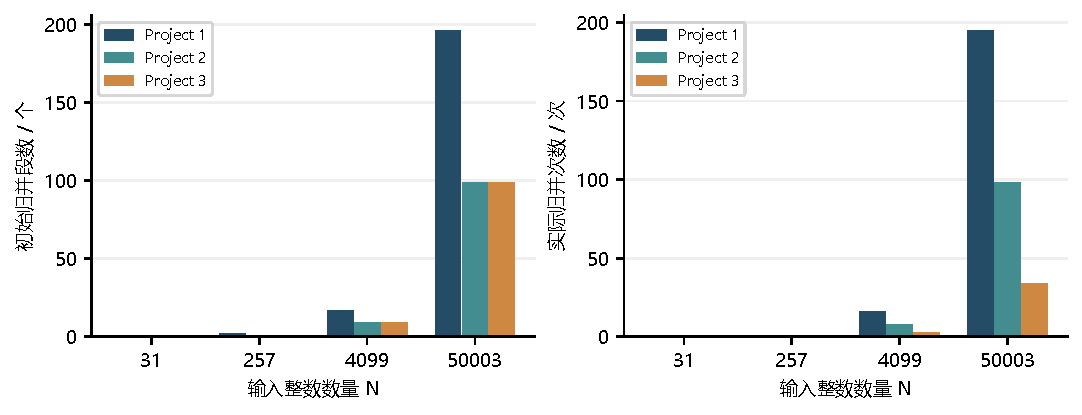
\includegraphics[width=\linewidth]{figures/runs-merges.pdf}\caption{Windows实测的初始段与归并次数；横轴按四个实验规模分类}\label{fig:runs-chart}\end{figure}

P2对99段二路合并98次，P3四路合并34次、4轮。只比较归并次数仍不充分，因为不同组处理的数据量不同，且部分单段直接带过。图\ref{fig:rounds-chart}单独给出P3轮数与阶段数，表明“轮数少”不等于“线程同步少”。
\begin{figure}[H]\centering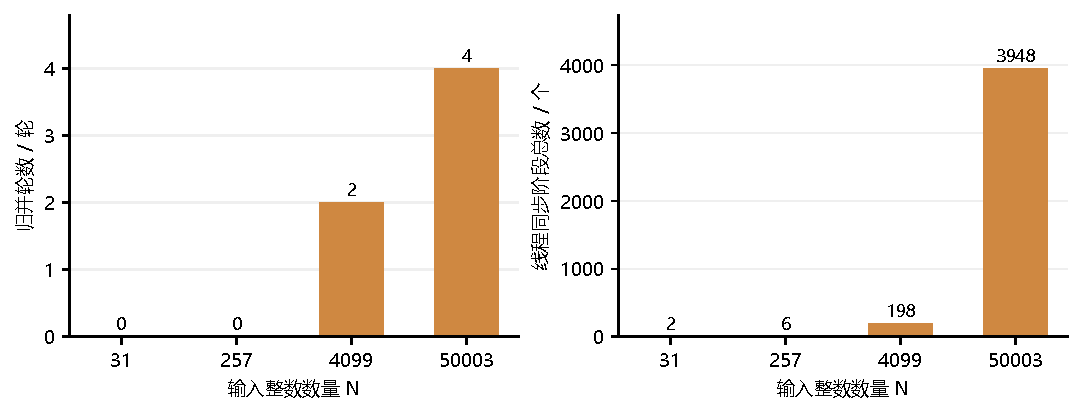
\includegraphics[width=\linewidth]{figures/rounds-stages.pdf}\caption{Project 3的归并轮数与三线程阶段总数，两个纵轴分别标注}\label{fig:rounds-chart}\end{figure}

默认15值下改变$k$也经过实际运行：$k=2$为2次归并、2轮，块读18、块写17；$k=3$与$k=4$都能把3个初始段一次合并，均为1轮、块读13、块写12。这里$k=4$仍分配8个输入块，但本组只有3路，说明配置容量与实际参与路数不同。

\subsection{数据块读写与实际时间}
图\ref{fig:io-time}比较最大实验规模的调用数，并展示四种规模的实际排序时间。$N=50003$时P1读写合计13964，P2为12258，P3为7970。P3相对P1减少约42.9\%的应用层数据块调用，但计时约为919.6 ms，高于P1的57.579 ms和P2的160.114 ms。

\begin{figure}[H]\centering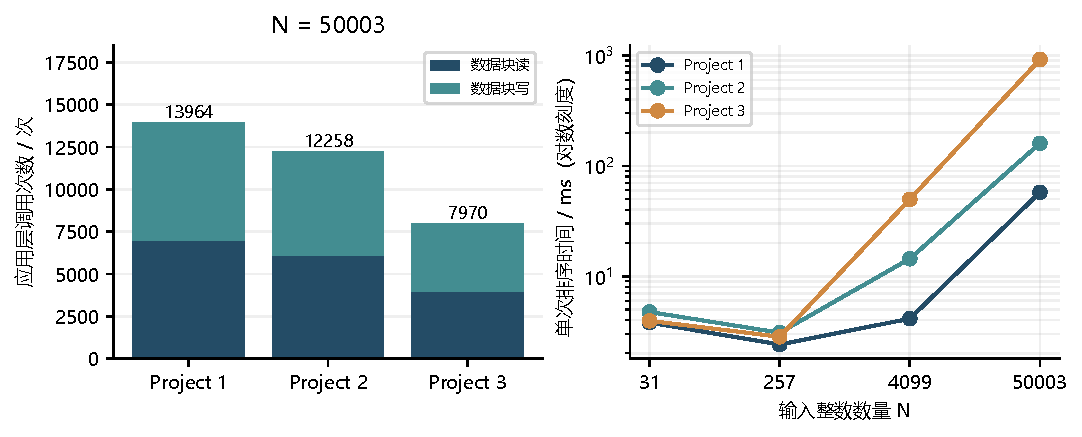
\includegraphics[width=\linewidth]{figures/io-time.pdf}\caption{Windows Release的数据块调用与单次耗时；时间纵轴使用对数刻度}\label{fig:io-time}\end{figure}

当前$B=64$仅为256字节，一个阶段产生的计算与I/O工作很少，而P3累计3948个同步阶段，每阶段新建并join三个线程。测试输入约200 KB，可被系统缓存，减少逻辑调用并不必然换来相应的物理磁盘节省。线程管理、调度和元数据操作可能占主导。这是对现象的合理解释，实验未单独测量每项开销，不能声称已精确分解各自占比。

\code{writes}不总等于\code{reads}：置换输出跨段时按段号分拆，K路缺头时可提前结束阶段并写出不足块的数据。小规模$N=31$时P2和P3执行同样的长段生成且无实际K路合并，单次时间仍不同，进一步说明不能把微小计时差异直接归因于算法结构。

\section{Windows与WSL的独立比较及解释边界}
\begin{table}[H]\centering\caption{$N=50003$时两环境的独立单次计时}\label{tab:platform-times}
\begin{tabular}{lrrr}\toprule 环境 & Project 1 / ms & Project 2 / ms & Project 3 / ms\\\midrule
Windows Release & 57.579 & 160.114 & 919.600\\
此前WSL Release & 21.4028 & 93.0083 & 379.418\\\bottomrule
\end{tabular}\end{table}

两份CSV除时间外，全部12行的段数、归并次数、轮数、块读写与阶段数逐项一致，支持算法行为在两种已测环境中一致。表\ref{tab:platform-times}不是操作系统性能排名：编译器、文件系统、缓存与运行时负载未被严格控制，不能把全部差异归于Windows或Linux本身。

同样$M,B,k$也不代表三项目总内存完全一致。P3持有更多输入块，置换选择有候选状态与段号标签，目录和计划随段数增长。最大输入50003个整数确实远超过候选容量256，能够触发多轮外排序流程，但尚未超过机器物理内存；不能将它描述为超大规模磁盘压力测试。

本实验支持的结论是：三种实现的正确性及课程机制在覆盖样本中得到验证；长段与K路归并减少了相关段数和应用层块调用；当前阶段线程实现并未在此测量条件下获得加速。更大的块、更多重复试验或线程复用可以作为后续研究，不能作为本报告已经完成的优化。

\chapter{实验总结}
\section{完成情况与证据链}
本实验完成Week 3--8的连续工程：底层能够创建、查询和流式追加不等长归并段；Project 1完成分块内排与后序二路计划；Project 2完成败者树置换选择、冻结解冻、三线程双缓冲与哈夫曼计划；Project 3完成共享$2k$输入池、动态预取、真正K路选择与多轮主控。

对机制的确认不只依赖最终排序结果。小例子给出段长、树节点、冻结标记和块号变化；独立断言检查一条路占用四块与跨路回收；220次端到端测试逐项对照完整参考排序；Benchmark每行也经过精确验证。Windows的九个具名配置、F5断点、F10单步、Ctrl+F5以及中文路径构建经过实际运行。源码注释最后独立提交，随后再次编译并通过Debug/Release完整验收。

\section{实际遇到的问题与解决过程}
\subsection{构建环境与编码差异}
起初Windows普通终端没有可调用的C++编译器，VS Code扩展本身也不提供编译器。先使用已存在的WSL GCC完成算法验证，后经用户确认安装微软Build Tools的必要C++组件，复用现有CMake。Windows使用Visual Studio多配置生成器，Debug和Release程序位于各自子目录；不能照搬Linux单配置目录中的程序路径。

PowerShell默认读取UTF-8中文材料曾显示乱码，改为显式UTF-8读取后恢复。原生MSVC编译保留\code{/utf-8}，中文脚本采用兼容Windows PowerShell的UTF-8 BOM，文档和源码保持UTF-8。解决办法是核对读写编码及实际编译日志，而非删除中文注释。此次报告中的源码快照仍保留所有中文说明。

\subsection{测试目录生命周期与文件系统开销}
此前WSL把大量微小I/O测试放在Windows挂载路径，Project 1阶段测试约97.7秒；改到Linux用户目录后，同类运行明显加快。因此原始WSL性能表明确使用Linux文件系统，不与挂载路径数据混合。另一次WSL空闲退出后\code{/tmp}构建目录消失，最终改用用户缓存目录，避免临时目录生命周期影响复现。

测试程序使用固定文件名，便于课堂演示和检查目录，但同一目录的多个进程会互相覆盖。当前一键验收顺序执行，Debug、Release及CTest使用明确的工作位置。目录隔离是实验条件的一部分，不应在无意并发运行后把文件冲突解释为归并算法错误。

\subsection{Ctrl+F5复用终端的工作目录}
实际GUI验收发现，C/C++扩展1.35.6在Ctrl+F5复用已有终端时未更新工作目录，可能将相对路径数据写到仓库根。F5调试子进程的目录正确，但终端Shell的提示符仍在原位置，单看提示符不能确认子进程的文件位置。

检查扩展实际行为后，采用最小的Windows入口兼容修正：具名启动配置传\code{--workdir DIRECTORY MODE}，程序先检查目录并切换，再沿用原模式解析。该修正只放在Windows条件编译分支，不改排序接口。中文目录成功、无效目录拒绝、缺参数拒绝均经测试；真实Ctrl+F5后运行目录文件更新时间改变，根目录旧文件保持不变。该修正与后续纯注释提交分开保存，避免把行为变化伪装成注释维护。

\subsection{接口连接、线程收尾和验证口径}
先前一次在旧构建仍运行时接入下一阶段源码，CMake源列表与引用短暂不同步，出现未链接\code{replacementSelection}；按完整列表重新配置构建后通过。最终回归期间先停止源码修改，再构建完整工程，避免用更新中的文件混合证明最终状态。

审查中为线程创建失败补充先join已启动线程的收尾，防止仍可连接的线程析构触发终止。没有故意制造线程资源耗尽，因此只陈述审查与正常运行验证。尾块、段边界和未知头值分别通过明确状态处理与独立测试覆盖；本报告不虚构曾发生的死锁或丢数事故。

验证口径也作了明确区分。自动生成输入能够完整对照\code{std::sort}；用户自定义大文件仅流式检查数量和非降序，并在输出中说明不是精确多重集合比较。保存的Benchmark计时不包含参考检查，不将“测试总耗时”当成排序时间，也不把应用层调用称为硬盘物理I/O。

\section{学习收获与验收理解}
本项目把排序中的抽象“序列”落实为文件中的连续区域。理解一个段不仅需要知道值的顺序，还要知道目录下标、段内元素位置和字节偏移的转换。\code{beginRun/writeBlock/endRun}使段长未知时仍能持续输出，缓冲区则让算法保持逐元素逻辑而文件保持分块访问。

归并计划与败者树解决的是两类不同问题。前者安排哪些段先合并，叶子是段；后者决定下一个输出哪个候选，叶子是当前值。哈夫曼计划优化加权搬移量，冠军路径重赛减少重复比较，置换选择通过冻结延长初始段。把它们混成一棵“排序树”会妨碍理解，按接口和生命周期区分后更容易解释复用关系。

线程部分最关键的是数据何时可见、由谁修改。预留块尚未入队，计算不能读取；耗尽块尚未同步，输入不能重用；新输出尚未完成，写线程不能访问。join不是装饰性等待，而是这些状态交接的边界。实际时间又说明，逻辑上存在并行任务，不意味着在小数据、小块环境下一定更快。

学习和验收时可沿同一15值输入追踪三个项目：先定位R0的物理偏移，再画普通计划，随后手算冻结与解冻，最后指出物理块2怎样跨路使用。报告与中文注释提供可检查依据；对函数的理解仍应通过自己预测下一步状态、修改参数并核对实际结果来巩固。

\section{局限性与改进方向}
\begin{enumerate}
\item 文件保留全部初始和中间段，便于观察但增加磁盘占用；尚无空间回收和压缩。
\item 文件结构采用本机字节序，未实现通用序列化、校验和与掉电恢复。输入输出须为不同真实文件，未处理所有路径别名或链接。
\item 候选和数据块受容量约束，目录、段号列表及计划仍为$O(R)$；并非恒定总内存系统。
\item 每阶段新建三个线程，未实现线程池或复杂异步调度。可考虑复用线程、扩大块并重复测量，但这些不属于已完成结果。
\item 未开展大于物理内存的长期磁盘压力测试，未验证磁盘满、真实掉电、跨字节序及系统线程耗尽。测试不能证明所有未覆盖故障路径。
\item K路每阶段扫描与重建树、段名线性查询及重复加载目录存在额外成本；后续若优化，应先保持机制与正确性测试，再单独测量收益。
\end{enumerate}

\section{材料来源与复现文件}
课程依据为用户提供的《外存数据管理》85页课件及两份课堂语音转写；六部分报告结构采用用户提供的Project Reports要求。原课件与讲稿仅供本地参考，未发布到公开仓库。本报告的架构图、算法图和说明按最终源码重新绘制和撰写。

实现依据为最终仓库17个C++文件、\code{README.md}及\code{docs/}中的讲义、课程对应、实验总结与验收问答。Windows与WSL数据分别来自\code{benchmark-windows.csv}、\code{benchmark.csv}；截图为真实Windows程序窗口。最后回归原始日志保存在本地\code{.local/windows/}，报告目录另外保留必要证据副本。

\code{report/README.md}给出XeLaTeX编译方法、源码快照生成方法和检查步骤。\code{scripts/build_report.ps1}执行编译与验证，\code{scripts/make_charts.py}从CSV生成矢量图。源代码附录紧接本章并位于整份报告末尾，包含最终实际实现及中文注释。

\chapter{完整源代码}\label{chap:source}
本章由脚本直接读取最终仓库文件生成，包含\code{main.cpp}、\code{src/}和\code{tests/}下全部正式C++头文件与实现文件，不以截图或省略号替代代码。每个文件保留完整中文注释、缩进和行号；较长语句按版心换行，行号仍按源码原始行计算。

快照对应Git提交：\par\noindent{\small\texttt{478a7ec6bcc95793a0e5540225609df04986bae2}}\par
正式C++文件共17个，另附CMakeLists.txt作为构建配置。


快照文件及SHA-256摘要保存在\code{code_appendix/manifest.json}。\code{scripts/snapshot_code.py}检查工作区与提交一致后复制源码，\code{scripts/verify_report.py}检查所有快照；普通重新编译不刷新快照，以保证报告的可复现性。
\Needspace{8\baselineskip}
\section{main.cpp}
\VerbatimInput{code_appendix/main.cpp}
\Needspace{8\baselineskip}
\section{src/buffer.cpp}
\VerbatimInput{code_appendix/src/buffer.cpp}
\Needspace{8\baselineskip}
\section{src/buffer.h}
\VerbatimInput{code_appendix/src/buffer.h}
\Needspace{8\baselineskip}
\section{src/kway\_merge.cpp}
\VerbatimInput{code_appendix/src/kway_merge.cpp}
\Needspace{8\baselineskip}
\section{src/kway\_merge.h}
\VerbatimInput{code_appendix/src/kway_merge.h}
\Needspace{8\baselineskip}
\section{src/loser\_tree.cpp}
\VerbatimInput{code_appendix/src/loser_tree.cpp}
\Needspace{8\baselineskip}
\section{src/loser\_tree.h}
\VerbatimInput{code_appendix/src/loser_tree.h}
\Needspace{8\baselineskip}
\section{src/merge\_plan.cpp}
\VerbatimInput{code_appendix/src/merge_plan.cpp}
\Needspace{8\baselineskip}
\section{src/merge\_plan.h}
\VerbatimInput{code_appendix/src/merge_plan.h}
\Needspace{8\baselineskip}
\section{src/projects.cpp}
\VerbatimInput{code_appendix/src/projects.cpp}
\Needspace{8\baselineskip}
\section{src/projects.h}
\VerbatimInput{code_appendix/src/projects.h}
\Needspace{8\baselineskip}
\section{src/replacement.cpp}
\VerbatimInput{code_appendix/src/replacement.cpp}
\Needspace{8\baselineskip}
\section{src/replacement.h}
\VerbatimInput{code_appendix/src/replacement.h}
\Needspace{8\baselineskip}
\section{src/run\_file.cpp}
\VerbatimInput{code_appendix/src/run_file.cpp}
\Needspace{8\baselineskip}
\section{src/run\_file.h}
\VerbatimInput{code_appendix/src/run_file.h}
\Needspace{8\baselineskip}
\section{tests/test\_sort.cpp}
\VerbatimInput{code_appendix/tests/test_sort.cpp}
\Needspace{8\baselineskip}
\section{tests/test\_sort.h}
\VerbatimInput{code_appendix/tests/test_sort.h}
\Needspace{8\baselineskip}
\section{CMakeLists.txt}
\VerbatimInput{code_appendix/CMakeLists.txt}

\end{document}
